\chapter{Power system security}
\label{ch:security}

\TODO{contingency types~\cite{ContingencyTypes}, future work: FMEA protection, missing vs unwanted trips., n-1-1 requires screening~\cite{VittalN-1-1}}

\TODO{timescale decomposition, Eurostag and Dynaflow examples}

\TODO{QSS comparison on ccdf of total risk in log scale, but does not compare critical contingencies / recommendations given for risk reduction}

As mentioned in the introduction, security is the ability of a power system to withstand disturbances arising from faults and unscheduled removal of equipment without further loss of facilities or cascading outages~\cite{AdequancySecurityDefinition}. Security is a complex problem, and many methodologies have been developed for the security assessment of power systems. Section~\ref{sec:traditionalSecurity} describes the ``traditional" (deterministic) security assessment methodology used by transmission system operators (TSOs) worldwide. Section~\ref{sec:probabilisticSecurity} then reviews different classes of probabilistic methodologies developed in the literature and discusses their limitations. Section~\ref{sec:security-conclusions} concludes with a discussion of the limitations of state-of-the-art assessment methodologies.

% As power system security is more and more threatened by dynamic phenomena, section~\ref{sec:stability} concludes this chapter with a review of the most important dynamic phenomena.


\section{Traditional security assessment}
\label{sec:traditionalSecurity}

In the traditional methodology, a power system is deemed secure if it can withstand a set of ``credible contingencies" without affecting customers nor violating security limits~\cite{N-1-ENTSOE}. The set of credible contingencies is often based on the famous N-1 criterion, i.e. the power system should be able to withstand the loss of a single element (out of N)\footnote{It should be noted that disconnections for maintenance are predictable and thus not considered to be contingencies. Disconnections for maintenance are thus already included in the N-0 situation.}.
% A contingency is an unpredictable loss of one or several elements of the network (lines, transformers, generators, etc.). Disconnections due to maintenances are thus not contingencies.
The possible loss of multiple elements due to a common mode failure (e.g. lines mounted on the same tower, lines connected to the same busbar) is a common addition to this list. The list definition varies from TSO to TSO and also on the considered time horizon (operation or planning). Also, during operational planning, the size of the list can vary depending on weather conditions. For example, the loss of multiple lines mounted on the same tower can be added to the list during a thunderstorm~\cite{N-1-ENTSOE}.

The definition of security limits also varies from TSO to TSO. Typically, security limits include a flat voltage profile (e.g. voltages at all buses between 0.95 and 1.05pu, this is to avoid disturbances for consumers and cascading outages), and the absence of overloads on all elements (to avoid cascading outages). Depending on the TSO, the security limits should be satisfied without the need for corrective actions (preventive approach) or after corrective actions have been implemented (corrective approach). In case (non-automated) corrective actions are used, it makes sense to define different security limits before and after the corrective actions are implemented (e.g. voltages between 0.9 and 1.1pu just after the disturbance, and between 0.95 and 1.05 after corrective actions).

A last important element of the traditional security assessment methodology is the set of pre-contingency states of the system whose security will be assessed. Close to real-time operation, the pre-contingency state considered can simply be the current state of the system as estimated by the SCADA system. During planning, this is more complex as one should consider load and intermittent generation variability, possible generators and transmission elements unavailability, etc. The set of pre-contingency states (and credible contingencies) should be defined according to the following criteria~\cite{CIGREreviewOfTools}.

\begin{itemize}
    \item Credibility: the pre-contingency states should be reasonably likely to occur.
    \item Severity: the pre-contingency states considered should lead to the worst-case performance of the system for the considered contingencies.
    \item Representativity: the pre-contingency states and contingencies considered should cover the main weaknesses of the system and phenomena observed during past outages.
\end{itemize}

With the growing installed capacity of renewable but intermittent energy sources, it is becoming more difficult to choose a set of pre-contingency states and contingencies that satisfy the above criteria. Indeed, the variability of renewable energy sources greatly increases the number of possible pre-contingency system states. Consequently, the number of possible system issues also increases. There is thus an increasing risk of missing ``worst-case scenarios". On the other hand, some issues might only appear during very specific system configurations. Designing the system around such issues would thus be uneconomical.


\section{Probabilistic security assessment}
\label{sec:probabilisticSecurity}

Probabilistic methodologies are based on the concept of risk. The risk of a scenario is defined as the product of its probability (of occurrence) and its consequences. The consequences are usually expressed as energy (in MWh) not served or as the monetary cost of such energy not served\footnote{It should be noted that the cost of energy not served is much larger than the cost of energy. For example, Ref.~\cite{VOLL} estimated the cost of a one-hour interruption of supply of a typical load to be around 20€/kWh. While the price of electricity on the bulk energy market is around 50€/MWh, so three order of magnitude lower.}. Risk is thus expressed in MWh/y or €/y. Probabilistic approaches allow to have a cost-benefit analysis of the measures (investment in new assets, redispatch, etc.) used to secure the system. So, probabilistic methods should lead to more economical planning and operation of power grids. Another advantage of those methods is that, as opposed to deterministic methods, it is not necessary to know a priori the ``worst-case" pre-contingency states and contingencies. When performing a probabilistic security assessment, one can use a larger set of states and contingencies. Then, the scenarios that contribute the most to the risk will naturally have a higher impact on the recommendations on how to secure the system. Disadvantages of probabilistic methods are however additional data requirements due to the necessity to estimate the probability of scenarios, and higher computation times due to the higher number of scenarios to simulate.

The necessity to transition from deterministic security assessment methodologies to probabilistic methodologies has been acknowledged in the industry and the literature. For example, the already-mentioned decision 07/2019 of the Agency for the Cooperation of Energy Regulators (ACER) of 19 June 2019 requires the European transmission system operators to develop a probabilistic approach for risk assessment of power systems by 2027~\cite{ACER}. In the literature, research on probabilistic security assessment has been active for more than two decades. The remaining of this section reviews the state of the art of probabilistic security assessment methodologies and compares the main types of methodologies available.

Actually, a lot of different methodologies can be placed under the umbrella of probabilistic methodologies, but the number of uncertainties taken into account can vary greatly. The most straightforward probabilistic assessment method is the contingency enumeration method. It is similar to the deterministic method in that one will assess the security of a list of contingencies (usually larger than in a deterministic assessment, e.g. including N-2 events and loss of towers). The difference is that contingencies are associated with a probability. Also, instead of simply classifying contingencies as acceptable or unacceptable, the consequences are usually computed, but in a deterministic manner. Due to the relative simplicity of the methodology and similarity with the deterministic method, it is implemented in most commercial software tools\footnote{At the time of the writing of the CIGRE review~\cite{CIGREreviewOfTools} (2010), all tools used the quasi-steady-state (QSS) approximation (that will be described in section~\ref{sec:QSSmethods}) to evaluate the consequences. Now, some tools (e.g. PSS/E~\cite{PSSE} and DIgSILENT PowerFactory~\cite{PowerFactory}) also allow to use dynamic simulations. Due to the simplicity of the method, it is possible to implement it with any tool that has basic scripting functionality.}~\cite{CIGREreviewOfTools}.

One industry-grade tool worth mentioning is ASSESS~\cite{AssessRTE, AssessNationalGrid} developed by RTE and National Grid (i.e. the French and British TSOs respectively). It does not compute the consequences of contingencies (i.e. only classify them as acceptable or not), but it generally consider more uncertainties in the pre-contingencies states, and it has a toolbox of statistic and data mining tools that can be used to analyse the results. It is particularly useful to define operational limits by ``drawing a line" between the acceptable and unacceptable pre-contingencies states.

\TODO{ASSESS: add fig? and keywork data mining}

A common mistake done when computing the probability of N-k events is to consider that it is equal to the product of the frequency of the k events. For example, ref.~\cite{CIGREreviewOfTools} says that if two lines have a failure rate of 1 in 20 years, then the double contingency failure is rate 1 in 400 years. This is however not true. The first way to understand why is to notice that the units do not match up. Indeed, the product of two frequencies should give a result in per squared years. A more intuitive way is to notice that the probability of two \textit{independent} failures to occur exactly at the same time (or in an infinitesimal time interval) is zero (respectively infinitesimal). One should thus define the size of the time interval during which failures are considered to be simultaneous. More rigorously, the rate of occurrence of a double contingency (in per year) is the product of the failure rate of one of the two assets (in per year) with the (probability of) unavailability (unitless) of the second. The unavailability of an element is given by:

\begin{equation}
\label{eq:availabilityMTTR}
    U = \frac{\text{MTTR}}{\text{MTTF} + \text{MTTR}}
\end{equation}

\TODO{Reformulate with \(\lambda_1(1-e^{-\lambda_2 T}) + \lambda_2(1-e^{-\lambda_1 T})\) to be more clear and correct, ref Haarla book, p67}

where the MTTR is the mean time to repair, and the MTTF is the mean time to failure of a component. Time to repair can vary greatly in power systems. For example, when a line has to be opened after a single-phase fault, it is often possible to automatically reclose it after a second or a few dozens of seconds (depending on the scheme used). When it is not possible (e.g. stuck breaker or no automatic reclosure scheme installed), it might be necessary to send crew to reclose the line which can take a few hours. Repair times of large assets (transformers, towers, etc.) can be several weeks.

It is important to note however that after the failure of an element, operators will try to perform corrective actions to bring the system back to a (N-1) secure state. If a second contingency occurs after corrective actions have been performed, this will be called a N-1-1 contingency. Corrective actions can typically be performed in 15 minutes. So the MTTR in eq.~\ref{eq:availabilityMTTR} should be replaced by \(\max(\text{MTTR}, 15\text{~min})\).

% It is common practice to assume that operators are able to secure the system in 15 minutes~\refs. So, two contingencies separated by more than 15 minutes are often referred to as N-1-1 contingencies instead of N-2 contingencies. To compute the rate of occurrence of N-k contingencies, one has thus to bound the time to repair by 15 minutes.
% Racourci de dire que > 15min => N-1-1


Double and higher order contingencies do not only occur due to the simultaneous occurrence of independent failures. Another important cause is the co-called hidden failures. A hidden failure is defined as a permanent defect that will cause a relay or a relay system to incorrectly and inappropriately remove a circuit element(s) as a direct consequence of another switching event~\cite{ZoneVulnerability}. Hidden failures are especially dangerous since they can cause high-order contingencies with a relatively high probability. For example, after a line fault, if one end of a line cannot be open, all lines that are connected to the same busbar or substation (depending on the cause of the failure, more details in chapter~\ref{ch:protections}) will have to be disconnected to clear the fault. This causes a N-k contingency (with k in the order of 2 to 10) whose probability can be several orders of magnitude higher than the probability of k independent failures. Also, as hidden failures usually cause the loss of adjacent elements, they tend to have higher consequences than the loss of independent lines that could be very far apart from each other.

\TODO{Mention Ian Dobson paper \url{https://ieeexplore.ieee.org/stamp/stamp.jsp?arnumber=10054456}, but (identified) critical lines might have more reliable protections (e.g. double differential (independent sets of relays), or even SIPS) than less critical ones (e.g. single distance protection with overcurrent backup). (Time resolution of data (1min) makes it difficult to differentiate between independent events and cascade. Actually, probably need some manual postprocessing to separate the two)

It turns out
for two North American publicly available historical outage data sets that the three
contingency motifs , , account for most of the probability of multiple line
outages [32].

https://iandobson.ece.iastate.edu/PAPERS/dobsonchapter2SPRINGER24.pdf

[32] K. Zhou, I. Dobson, Z. Wang, The most frequent N-k line outages occur in motifs that
can improve contingency selection, early access in IEEE Trans. Power Systems, 2023. doi:
10.1109/TPWRS.2023.3249825



}


The importance of hidden failures is highlighted by the study of historical blackouts. For example, Ref.~\cite{CascadingMethodoAndChallenges} observed that out of the 26 major unreliability events reviewed in a CIGRE (Conseil international des grands réseaux électriques) report\footnote{Most of these disturbances affected more than one million customers and led to at least 5~GW of unserved power}~\cite{majorBlackouts}, 19 of them were triggered by losses of single transmission elements albeit many of these events were exacerbated by other problems. Further analysis shows that 18 of the 26 events were caused or aggravated by hidden failures. The same observation can be made for smaller scale events. For example, the study of significant disturbances reported by the NERC~\cite{NERCDisturbancesReport} (North American Electric Reliability Corporation) in the period from 1984 to 1988 and summarised in~\cite{ZoneVulnerability} indicates that protective relays misoperations were involved, in one way or another, in 73.5\% of disturbances\footnote{This include both spontaneous operation of protections (without preceding event) and hidden failures. However, as power systems are designed to be N-1 secure, spontaneous operations should usually not have consequences.}.


Industry-grade tools only consider the uncertainties related to the initial state and initial contingencies. After the occurrence of a given contingency, the system is simulated in a fully deterministic manner. Those tools are thus unable to consider hidden failures as those manifest after the initial contingency\footnote{The hidden failures that occur just after the initiating event (e.g. failure to open a faulted line) could be modelled as part of the initiating events as done in~\cite{Haarla, GridPSA}. This is discussed in section~\ref{sec:DynMethods}. This is however not possible for failures that occur later in the cascade. For those, it is necessary to have a probabilistic simulation of the evolution of the cascade.}.

Another limitation of modelling cascading outages in a deterministic manner is that cascading outages tend to have a ``chaotic"\footnote{Not stricto sensu} behaviour. This is because in a cascading outage, many elements are subject to abnormal conditions and thus likely to trip or misoperate. A good example of this is the tripping of lines caused by overload. When a line is overloaded, its temperature increases due to the Joule effect. It thus sags and can then enter in contact with vegetation causing a short-circuit followed by a trip of the line. The line trip causes a redistribution of the power flows and can cause overloads in other lines which contribute to the propagation of the cascade. The redistribution could also resolve some overloads, stopping the cascade propagation. In a deterministic simulation, it is a common assumption to consider that when multiple lines are overloaded, the line with the most severe overload will trip first. In practice, slightly less overloaded lines could trip first due to different vegetation height, weather, etc. The trip of a different line can cause a very different redistribution of power flows that causes different lines to be overloaded in the next step of the cascade. The resulting cascade can thus be very different (in terms of size, geographical distribution, impacted elements, etc.) than the one simulated in a fully deterministic way. This difference is further amplified when we consider the competition between different cascading mechanisms.

These limitations of deterministic methods have fostered the development of probabilistic methodologies that are reviewed in the remaining of this section. Two main categories of probabilistic methodologies exist. The ones that use a static grid model (section~\ref{sec:QSSmethods}) and the ones that use a dynamic grid model (section~\ref{sec:DynMethods}). These methods are quite different as they have to cope with different limitations. The former have to introduce additional methods to approximate dynamic effects while the latter are limited by computation times. Additionally, section~\ref{sec:OtherMethods} reviews other types of methods that do not fall in the previous categories.


\subsection{Methods with a static grid model}
\label{sec:QSSmethods}

Methods based on a static grid model, often referred to as quasi-steady-state (QSS) methodologies typically follow the same procedure~\cite{Benchmarking2018}. First, the system is initialised at the pre-contingency state, and the initiating contingencie(s) are triggered. Then, the post-contingency state is computed using a load flow algorithm. If some elements are subject to unacceptable conditions (e.g. overload, undervoltage, etc.), those elements are tripped or other remedial actions are implemented (e.g. under-voltage load shedding (UVLS), redispatch, etc.). After those disconnections/actions, the state of the system is recomputed. The process is repeated until no more elements are subject to unacceptable conditions or if a full blackout occurs.

The IEEE Working Group on understanding, prediction, mitigation and restoration of Cascading Failures (WGCF) classifies QSS methodologies according to five dimensions listed below~\cite{Benchmarking2018}. It should be noted that some of these dimensions are themselves not one-dimensional.

\begin{itemize}
    \item Pre-contingency states: most methodologies assess the risk of the system for a single pre-contingency state. The two most common extensions are the risk assessment over a given time period (e.g. one year, to consider e.g. seasonality of the load, maintenances, etc.), and inclusion of uncertainties (e.g. renewable generation). Uncertainties are generally treated using Monte Carlo (MC) methods. Ref.~\cite{PSAreviewPreeceMilanovic} reviews the most common probability distribution used to model different kind of uncertainties, as well as various methods used to overcome the limitations of basic Monte Carlo (e.g. sequential MC and Markov chain MC can be used to model dependencies between uncertain variables and time dependence, while importance sampling and quasi-MC can be used to increase the effectiveness of MC). It should be noted that pre-contingency sampling methods are roughly the same for methods with static and dynamic grid models. The paper thus reviews all of them.
    \item Degree of stochasticity: this includes both initiating and subsequent events.
    \begin{itemize}
        \item Initiating events: in a deterministic approach, all N-k initiating events of a given order are considered, although a probability can be associated to each a posteriori. In a probabilistic approach, their probability is considered in the sampling process.
        \item Subsequent events: in a deterministic approach, the evolution of the cascade is based purely on deterministic thresholds. For example, if a line is overloaded beyond a predefined limit, it is always disconnected\footnote{In case of simultaneous (in the QSS sense) violations, either the element with the worst violation is disconnected, or all elements with violations are disconnected}. This leads to a single possible evolution of the cascade for a given initiating event and pre-contingency state. In a probabilistic approach, elements are given a probability to trip when they are subject to violations (the probability can depend on the severity of the violation and other factors). For a given contingency and pre-contingency state, one thus obtains multiple cascading paths, each associated with a probability and specific consequences.
    \end{itemize}
    \item Population of the contingency list: different methods can be used to generate the contingency list. The most common are contingency enumeration (consider all N-k contingencies up to a given order) and MC sampling. The contingency list can be reduced to the contingencies most likely to cause cascading failures by using screening methods.
    \item Power flow model: the pre-contingency state can be modelled either with an AC (full) or a DC (linearised) power flow. The DC model is faster but unable to account for voltage issues. Different methods can also be used to solve possible violations and non-convergence issues (of the AC load flow) in the post-contingency states. For example, an optimal power flow (OPF) will tend to model the actions that operators would use to solve the violations. The possible actions considered in the OPF can be load shedding, redispatch, topological actions, etc. Another possibility is to use models of protections such as UVLS, overcurrent protections of lines and transformers, etc. Some tools simply assume a total blackout in case of non-convergence of the load flow.
    \item Cascading mechanisms modelled: the tripping of overloaded elements is included in all methodologies. The disconnection of load and/of generators in case of unacceptable voltage is also commonly seen. Methodologies that consider hidden failures are a bit rarer\footnote{Also, as will be discussed in chapter~\ref{ch:protections}, dynamic grid models are required to model some hidden failures.}. Finally, dynamic cascading mechanisms (e.g. frequency, angle, and voltage stability issues) have to be modelled in a simplified way or using heuristics, and are considered by some methodologies.
\end{itemize}

In order to better illustrate QSS methodologies and the limitations in their modelling (especially dynamic issues), an example of QSS methodology is described and discussed. The example considered is the AC cascading failure model (AC-CFM)~\cite{ManchesterNoebels} that can be considered as one of the spiritual successors of the famous Manchester model~\cite{OriginalManchesterModel}. This model follows a similar procedure to most QSS models, that is it initialises the system, triggers a initiating contingency, and then checks for violations and performs corrective actions until all violations are solved. However, as most QSS models, it differs by the corrective actions modelled. The steps that are taken to solve violations at a given step of the cascade are illustrated in Fig.~\ref{fig:NoebelsFlowchart} and discussed below.

\begin{figure}
    \centering
    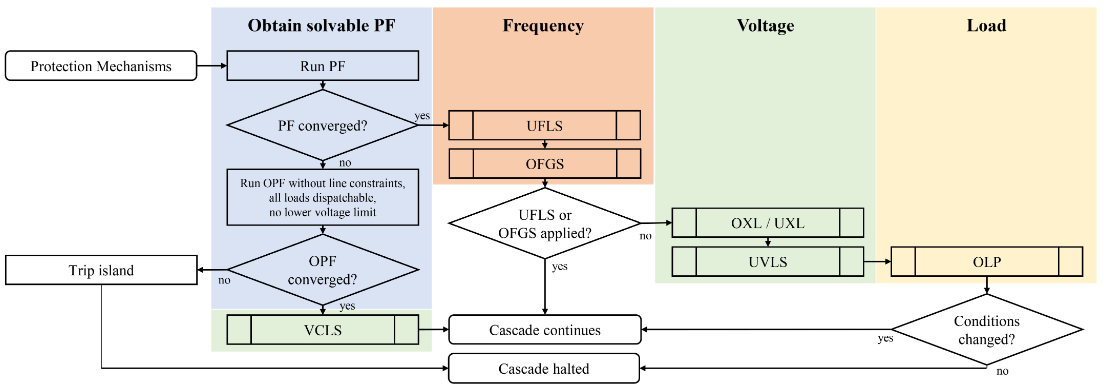
\includegraphics[width=\linewidth]{Figs/NoebelsFlowchart.png}
    \caption{Flowchart of the AC-CFM methodology~\cite{ManchesterNoebels}. Abbreviations: PF: power flow, VCLS: voltage collapse load shedding, UFLS: under-frequency load shedding, OFGS: over-frequency generator shedding, OXL/UXL: over/under-excitation limiter, UVLS: under-voltage load shedding, OLP: overload protection}
    \label{fig:NoebelsFlowchart}
\end{figure}

\TODO{Simplify figure to have less things to explain. In general, make text less dense.}

\begin{itemize}
    \item Obtain a solvable power flow: as the AC-CFM uses an AC power flow, the power flow can fail to converge. This is often caused by lack of reactive power support that causes a voltage collapse. The modelling choice made for the AC-CFM is to use an OPF considering all loads are dispatchable, and to minimise the load shedding necessary to obtain a converging load flow. In a dynamic simulation, voltage collapses occur in a ``smoother" manner as time is explicitly considered as a continuous variable. One can thus observe e.g. which loads are subject to undervoltages first and thus which UVLS relay actually triggers\footnote{Numerical stability issues can also occur in dynamic simulations but they tend to be rarer. To avoid those issues, one should be cautious of the models used (e.g. Ref.~\cite[p93-98]{SongThesis} proposes to replace constant-power loads with restorative loads with a very short time constant). Protections tend to mitigate numerical issues as they disconnect elements are subject to severe conditions (e.g. distance protections disconnecting lines during voltage collapse).}.
    \item Frequency: AC-CFM considers that if load-generation imbalances are less than a predefined threshold, the imbalance will be redistributed to the generators (that will increase or decrease their power to restore the imbalance) according to their participation factors. For larger imbalances, load or generation shedding\footnote{Generation shedding is most often called generator rejection, but the terminology of~\cite{ManchesterNoebels} is kept in this paragraph.} is necessary. In case of lack of generation, the load is reduced uniformly (although prioritisation can be implemented). In case of generation surplus, generating units are disconnected starting with the smallest ones as they tend to more easily lose synchronism. Also, the same imbalance threshold is used for all steps of the cascade. This is equivalent to assume that the frequency can be restored to its nominal value between each step. In a dynamic simulation, the evolution of the frequency is explicitly modelled. So, the maximum imbalance that does not cause load or generation shedding is the maximum imbalance that does not cause the frequency not to reach the threshold of under-frequency load shedding (UFLS, typically 49~Hz in a 50~Hz-system) or generator over-speed relays (typically 52.5~Hz). This maximum imbalance thus depends on the initial value of the frequency, the inertia of the system, potential synchronisation issues, etc. Also, for large imbalances, there is no guarantee that the balance can be restored before the frequency drops too low and generators are disconnected by their under-speed protections (typically at 47.5~Hz). This is especially true for systems with low inertia, for example, islands formed by the splitting of the original system, and/or systems with large penetration of (grid-following) renewable energy sources.
    \item Voltage: this block has two parts: the over/under-excitation limiters of generators, and UVLS. 
    \begin{itemize}
        \item OXL/UXL: in AC-CFM, generators that are over/under-excited are made into PQ buses, i.e. their reactive power output is considered equal to its limits. In a dynamic simulation, limiters would be modelled in a similar way. However, as over-excitation limiters protect the generators against excessive heating, a time-delay can be considered. It is also easier to consider the variation of reactive limits with the active power output.
        \item UVLS: in AC-CFM, load is shed by block until voltages reach acceptable values. If multiple loads are subject to undervoltages, load is shed in all of them simultaneously. In a dynamic simulation, the order of triggering of UVLS relays will depend on the time evolution of voltages at individual load buses. UVLS at one bus can then alleviate or worsen voltage issues in neighbouring buses.
    \end{itemize}
    \item Load: in AC-CFM, overloaded lines are tripped. If multiple lines are overloaded, they are all disconnected. In dynamic simulations, the order of tripping can be better modelled. Also, distance and out-of-step protections can be added in a dynamic model.
\end{itemize}

Additionally, the AC-CFM considers that frequency issues are solved first, followed by voltage issues, then overload issues. Again, in a dynamic simulation, the order and interactions between those issues can be better modelled. Finally, angle stability issues are not considered in AC-CFM.

The above discussion presented a particular QSS methodology with a given set of assumptions. However, for each of the cascading mechanisms, different assumptions could have been made. There is currently no consensus on the details of modelling required for QSS cascading failure simulation~\cite{Benchmarking2018, BenefitsAndChallengesDynamicPreece}. Also, the necessary level of detail is likely to be different for different systems and different operating conditions. Moreover, benchmarking has shown that different QSS methodologies lead to different results~\cite{Benchmarking2018}. In particular, the distribution of cascading sizes and the critical elements differed depending on the methodology used. Finally, comparison between a QSS and a dynamic simulator has shown similar behaviour during the early stages of the cascade (slow phase), but different results for the later stages (fast phase)~\cite{BenchmarkingStaticVsDynamic}. As purely fast cascades and dynamic issues are becoming more common~\cite{cascadeAcceleration}, the use of dynamic models is expected to increase in the near future.

Outside of the field of cascading outage analysis, there has also been some concerns regarding static grid models. For example, RTE (the French TSO) is developing a tool called DynaFlow for steady-state computations using simplified time-domain simulation. Steady-states are usually computed with a power flow algorithm. Additional loops are added on top of this power flow to account for controls used in power systems (e.g. on-load tap changers, phase-shifter transformers, etc.). The order or which those loops are applied has an impact on the final state that is computed. This order was previously defined using heuristics and experience, but this was becoming complex with the increasing number of loops, especially for large systems. DynaFlow showed more accurate results and ease of use~\cite{DynaFlow}. A similar tool called DynaWaltz was developed for long-term voltage stability. This tool replaced their previous QSS tool. DynaWaltz showed better accuracy than its predecessor while keeping similar computation times~\cite{DynaWaltz}. Note that both tools are deterministic.


\subsection{Methods with a dynamic grid model}
\label{sec:DynMethods}

Methods based on a dynamic grid model use time-domain simulations\footnote{In this thesis, time-domain simulations are implicitly assumed to use the root mean square (RMS) approximation. Dynamic methods are already strongly limited by computation time and thus cannot afford to use electromagnetic transient (EMT) simulations. Also, it is expected that the RMS approximation will remain adequate for most scenarios in the future~\cite{GridFormingAreTheyTheKey, AvoidEMT}.} to assess the consequences of a given scenario. Dynamic methods have been recognised as the most comprehensive and accurate methods for representing cascading outages~\cite{BenchmarkingStaticVsDynamic, BenefitsAndChallengesDynamicPreece, SongPaper}. The comprehensive aspect is maybe important to emphasise. Indeed, as illustrated in section~\ref{sec:QSSmethods}, QSS methods need to introduce heuristics and/or simplifications to account for dynamic phenomena, and to estimate the order of occurrence of static issues. As dynamic methods use similar models than in traditional dynamic stability assessment, the same largely accepted approximations can be reused (e.g. models of generators, exciters, etc.) which should help with the acceptance of dynamic security assessment methods by TSOs. The main difference between dynamic simulations for cascading outage simulations and stability assessment is that during cascading outages (i) the system is further from normal operation challenging the accuracy of the models, and (ii) protections (and their possible failure) play a much more significant role. Sensitivity studies are thus very important to control the first point. Chapter~\ref{ch:protections} is dedicated to the second.

The drawback of dynamic methods is significantly larger computation times\footnote{Traditional offline dynamic security assessment (that takes into account uncertainty of the pre-contingency states but no uncertainty after the initiating event) of real-scale systems can already take one day in a high-performance computing (HPC) environment~\cite{EurostagHPC}. A probabilistic dynamic security assessment would require even more computational power. The magnitude of the increase depends on the range of uncertainties considered and the efficiency of the method.} and data requirements. Compared to QSS methods, the additional necessary data are mainly linked to (i) the dynamic models of generators, loads, etc. and (ii) the models of protections. Data for the first point is generally available to TSOs as stability studies are performed routinely. However, it is important to have efficient data handling (e.g. automated transfer of data from stability tools to security assessment tools). The second point requires data regarding the failure rate of protections (that can be difficult to estimate) and the protection settings (that should be available but introduce additional data handling issues). Data requirements for dynamic security assessment are discussed in more details in section~\ref{sec:DataRequirementsForDSA}.

Multiple methods have been developed for probabilistic dynamic security assessment and are reviewed in the remaining of this section. In~\cite{SongThesis, SongPaper}, random N-2 failures are simulated using a custom simulator. Protections are modelled; however, they are assumed to be perfectly reliable. Ref.~\cite{Preece1000RandomDynN-2} uses a similar methodology but uses the commercial simulator DIgSILENT PowerFactory.

Ref.~\cite{Haarla, GridPSA} proposed a methodology based on event trees. An example of event tree is shown in Fig.~\ref{fig:eventTree}. An event tree starts at a given initiating event (a permanent line fault in the left of the figure). The event tree then branches when subsequent events (typically protections against the initial event) are possible. Upward branches are usually associated with the occurrence of an event (e.g. protection operates successfully), and downward branches with the non-occurrence of the event (e.g. protections fails to operate). The event tree thus generates a number of scenarios whose frequency and consequences can be estimated. In~\cite{Haarla, GridPSA}, the frequency is computed as the frequency of the initial event multiplied by the probability of the subsequent (non-)events. To complement event trees, fault trees can be used to model common-mode failures, they are presented in more details in dedicated literature, e.g.~\cite{FaultTreeHandbook}. Consequences are estimated using dynamic simulations. The limitation of this method is that the event tree is built prior running the simulations. The analyst thus has to predict what protections will be activated. In practice, this is only possible for the protections that isolate the fault (e.g. distance protections at both sides of the line and backups for these protections).

\begin{figure}
    \centering
    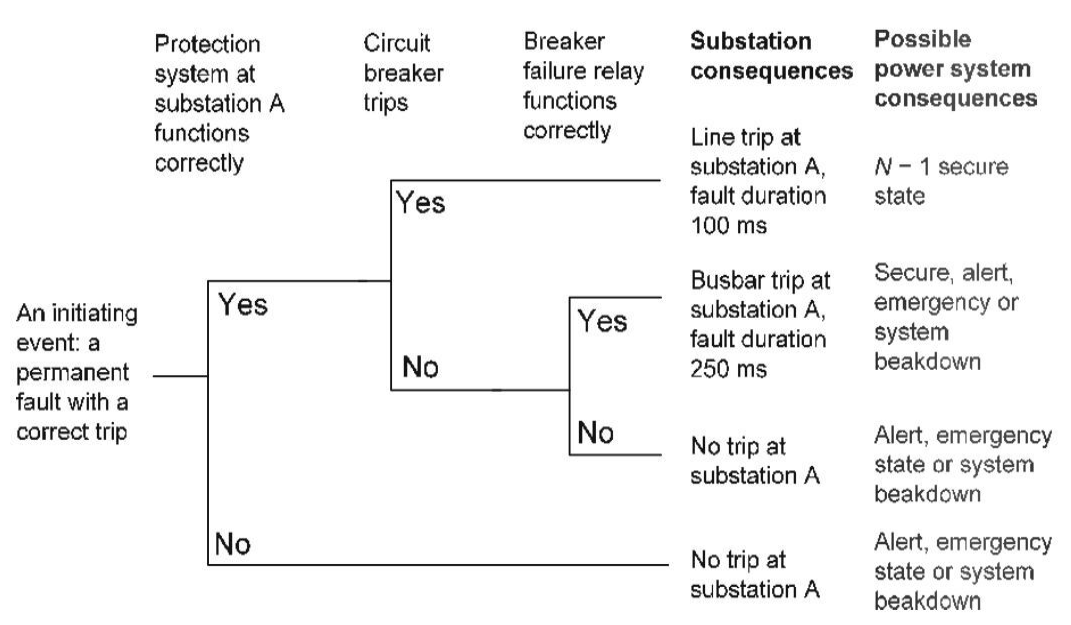
\includegraphics[width=0.8\linewidth]{Figs/EventTree.png}
    \caption{A simplified example of event tree for a line short-circuit~\cite{GridPSA}}
    \label{fig:eventTree}
\end{figure}

The Pacific Northwest National Laboratory (PNNL) developed a tool called Dynamic Contingency Analysis Tool (DCAT) for security assessment of power systems~\cite{DCATphase1, DCATphase2}. In this tool, after the initiating contingency, the evolution of the system is computed using dynamic simulation. Protections are modelled explicitly in the simulation, and when one protection activates, the simulation is stopped and the state of the system is saved. From this save, two simulations are run, one where the protection actually operates, and one where it fails to. The limitation of this method is that only missing protection operations are considered. Unwanted operations are not considered. Also, protections are considered perfectly accurate. The variable order of protection (due to e.g. measurement inaccuracies, incorrect settings, etc.) operations during a fast cascade is thus not considered. Finally, the reports did not show any example of application using the ``protection misoperation" functionality. There was also no discussion on the impact on the computational burden of this feature.

An interesting feature of DCAT is that is uses both dynamic and QSS simulations. Indeed, it uses dynamic simulations for the first 30 to 60 seconds after the initial contingency. If the system is deemed dynamically stable (i.e. if no event occurs during the last dozen of seconds of the dynamic simulation), the tool then switches to (deterministic) QSS simulation. When an event occurs in the QSS simulation (e.g. a corrective action), the tools switches back to dynamic simulation.

Ref.~\cite{PierreIEEEtran} proposes the use of dynamic event trees (DETs). DETs are an extension of event trees. In a DET, branchings are not predefined by the analyst but can occur at any time and any order. As time is a continuous variable, this means that a DET contains in principle an infinite number of scenarios. Numerical schemes are thus required to approximate those DETs. A more rigorous introduction to DETs is done in section~\ref{sec:dynamicReliability}. Ref.~\cite{PierreIEEEtran} proposed two numerical schemes. The first is skeleton-based MC. In this methodology, the first step is to build a so-called skeleton. This is done in a similar way as in DCAT, i.e. the evolution of the system is simulated, and when a protection is triggered, the simulation branches. In one branch, the protection actually operates, and in the second it fails to. Upon this skeleton, additional branches are grafted at discrete time steps before and after the original branchings points. These additional branches take into account measurement and setting errors of the relays. The probability of each of these additional branches depends on the evolution of system variables in the skeleton. For example, if the variable monitored by the protection ``hugs" the triggering threshold, the protection will be likely to trigger in a large time interval around its triggering time in the skeleton. On the other end, if the variable quickly goes beyond the threshold, the interval will be narrower. This methodology has been applied in~\cite{Faghihi}. The second method is MCDET. MCDET is a concatenation of MC and DDET (discrete DET, that can here be read as a synonym of skeleton\footnote{DDETs and MCDET are introduced more rigorously in section~\ref{sec:dynamicReliability}}). It was originally proposed in the nuclear domain by~\cite{MCDET}. In MCDET, continuous uncertainties (e.g. measurement errors) are handled by MC. Then, for each MC sample, a skeleton is built. This skeleton handles the discrete uncertainties (e.g. protection fails to operate). This method was however not fully implemented, and only preliminary results were presented~\cite{PierreMCDETprelim}.

\TODO{Define correctly MCDET (no skeleton)}

DETs are more powerful than the previously mentioned methodologies as they can in principle account for any kind of uncertainties. However, they tend to be even more computationally expensive, and require more interactions with the simulator. They are thus used with custom simulators or simulators with powerful APIs.

It can be noted that, like DCAT, Ref.~\cite{PierreIEEEtran} uses both dynamic and QSS simulations but with a different approach. The approach is based on the observation that most cascades can be divided in two phases. In the first phase, the cascade is driven mainly by thermal effects (line overloads, etc.) and can last up to several hours (so-called slow phase). At some point, electromechanical phenomena become dominant and cascade ends is a fast collapse (so-called fast phase that last from several seconds to several minutes). Likewise, the methodology has two parts. In the first phase, the slow phase is simulated using a probabilistic QSS methodology. When a possible dynamic instability is detected, the method goes to the second phase. In the second phase, DETs are used as described above. As the QSS methodology generates a large number of similar scenarios, those scenarios are aggregated before being fed to the second phase.

% \cite{QimingChenThesis} % Not fully clear what he does

% \cite{MultiTimescaleMarkovianTree-ActuallyOnlyQSS}

\subsection{Other methods}
\label{sec:OtherMethods}

As previously mentioned, QSS methods have to make difficult modelling choices to consider dynamic phenomena and to model the order of occurrence of static issues. This led some researchers to develop methods based on historical data. Indeed, historical data are by definition not dependent on modelling assumptions. From historical data, one can observe what elements played critical roles in past cascades. Those elements are good candidates for upgrades or replacements. However, historical data alone does not allow to perform ``what if" evaluation. For example, the benefits of a given upgrade cannot be estimated. This has led to the development of influence graphs models~\cite{CascadingInfluenceGraph} that are tuned to match historical data. The most famous model of this category is the Oak Ridge-PSERC-Alaska (OPA) model~\cite{OPA2019}. The issue when building models from historical data are that these data consist mainly in small cascades as large blackouts are (hopefully) rare. However, as previously mentioned, large blackouts although rare have a very important contribution to the total risk (e.g. of load shedding)~\cite{CascadingMethodoAndChallenges}. Moreover, large blackouts tend to be driven by different phenomena than small cascades. Indeed, large blackouts consist more and more often purely of a fast phase (driven by electromechanical phenomena), while small cascades always have an important slow phase (driven by thermal phenomena)~\cite{cascadeAcceleration}.

% \cite{TopologicalModelsBad}

A lot of machine learning techniques have been developed for dynamic risk assessment and are reviewed in~\cite{MLEfthymios}. However, those tools are only able to predict if a given scenario is stable or not (some tools are not purely dichotomic and can give a stability index or distance to stability indicator). They are thus unable to predict the consequences of a given scenario. Moreover, those tools are deterministic. For a given pre-contingency state and contingency, they only give one output. They are thus unable to generate new scenarios as done in a DET. % A potential application of machine learning for cascading outage analysis is as a screening method, i.e. a method to predict which scenarios are      % No because N-1 will often be stable, and need DET (or ET like Haarla might be enough?) to generate N-2


\section{Conclusion}
\label{sec:security-conclusions}

Two main types of methods for probabilistic security assessment of power systems were reviewed. The first type of models uses the QSS approximation, i.e. it simulates the evolution of the power system using a sequence of steady-states. Those methods require a large number of assumptions in order to handle power flow convergence issues and to model dynamic issues and the order of activation of corrective actions. There is currently no consensus on what hypotheses are acceptable to make, and different QSS methodologies have shown to give different results~\cite{Benchmarking2018}. Also, those methods are unable to accurately model fast cascading outages~\cite{BenchmarkingStaticVsDynamic}.

The second type of models is based on time-domain simulations. These methods are more accurate but require more computational power and input data. Out of the reviewed methodologies, DETs are the most powerful as they can in principle consider any type of uncertainty. However, they are even more computationally expensive than the other methods. Protections (and their potential failures) play a key role during cascading outages (especially fast cascading outages). They are thus naturally in a central position in all reviewed dynamic methods. However, only a few failure modes are considered in existing methodologies. This is discussed in more details in chapter~\ref{ch:protections} and~\ref{ch:SPS}. The issue of computation time is tackled in chapter~\ref{ch:DPSA}.

\TODO{As apposed to nuclear, no failure (except if already present) during system evolution}

\TODO{Can generate initiating event contingency list from historical data instead of my ``fault clearing event tree": https://arxiv.org/pdf/2209.02192.pdf (and add a few random N-2?, paper say 81\% of N-2 are adjacent lines, and 19\% remaining)}